\documentclass[a4paper,11pt]{article} 
\usepackage[spanish]{babel}
\usepackage[utf8]{inputenc}
\usepackage{authblk}
\usepackage{hyperref}
\usepackage{multicol}
\usepackage[version=4]{mhchem}
\usepackage[pdftex]{graphicx}
\usepackage{wrapfig}
\usepackage{appendix}
\usepackage{floatrow}
\usepackage{xcolor}
\hypersetup{colorlinks=true,linkcolor=blue,filecolor=magenta,urlcolor=blue,citecolor=green}

\providecommand{\keywords}[1]{\textbf{\textit{Palabras clave---}} #1}

\begin{document}
	\title {\bf Minerales super-reducidos en ofiolitas: No siempre una evidencia de manto profundo. El ejemplo de Cuba Oriental}
	\author[1]{\sl \bf Núria Pujol-Solà}
	\author[1]{\sl Joaquín A. Proenza}
	\author[2,3]{\sl Antonio Garcia-Casco}
	\author[2]{\sl José María González-Jiménez}
	\author[4]{\sl Vanessa Colás}
	\author[1]{\sl Àngels Canals}
	\author[1]{\sl Joan Carles Melgarejo}
	\author[2,3]{\sl Fernando Gervilla} 
	\affil[1]{Departament de Mineralogia, Petrologia i Geologia Aplicada. Universitat de Barcelona.}
	\affil[2]{Departamento de Mineralogía y Petrología. Universidad de Granada.}
	\affil[3]{Instituto Andaluz de Ciencias de la Tierra, CSIC-UGR, Granada.}
	\affil[4]{Instituto de Geología, Universidad Nacional Autónoma de México.}
	\renewcommand\Authands{ y }
	\date{}
	\maketitle
	\begin{abstract}
	\href{https://github.com/nurpss/proyecto_final}{https://github.com/nurpss/proyecto\_final}
	\\Este trabajo presenta los resultados obtenidos tras el estudio de muestras de cromitita y rocas asociadas (gabros y dunitas) en la transición manto-corteza de las ofiolitas de Cuba oriental. Los resultados sugieren que las fases super-reducidas en las rocas ofiolíticas se formaron a baja presión y baja temperatura durante el proceso de serpentinización.
	{\color{red} {\sl (***Se ha usado un texto y las imágenes de un abstract presentado como base, con modificaciones para poder usar las diferentes herramientas aprendidas durante el curso).}
	\end{abstract}
	
	\keywords{cromitita, moissanita, olivino, manto}
	 \\
	 \tableofcontents
	\begin{multicols}{2}
		\section{Introducción}
		En los niveles mantélicos de varios complejos ofiolíticos (p. ej.: China, Tíbet, Rusia, Turquía, Albania) se han encontrado recientemente minerales indicadores de condiciones de ultra-alta presión (\textgreater10 GPa y \textgreater300 km; p. ej. diamante, pseudomorfos de coesita y stishovita) y de condiciones super-reducidas (de 4 a 7 órdenes de magnitud por debajo del tampón IW; p. ej. elementos nativos, aleaciones, carburos, nitruros y fosfuros) que se suponen propias del manto profundo, junto a minerales formados típicamente en la corteza continental (p. ej. circón, cuarzo, andalucita, cianita, etc.). El origen de esta compleja asociación mineral es actualmente un tema de intenso debate, con varios modelos propuestos: reciclaje en niveles profundos del manto, plumas mantélicas, contaminación de la placa subducente, impacto de rayos de tormenta y plumas frías \cite{Pujol-Sola2018,Xiong} y referencias en estos artículos. 
		\section{Contexto geológico}
		En la parte más oriental de la isla de Cuba se encuentra el macizo ofiolítico cretácico de Moa-Baracoa \cite{Iturralde}, el cual se caracteriza por la preservación de una zona de transición manto-corteza (MTZ, por sus siglas en inglés) bien desarrollada. La MTZ se compone de harzburgitas, dunitas, peridotitas impregnadas (clinopiroxeno y plagioclasa) y diques y sills de gabro. En esta zona se encuentran numerosos cuerpos de cromititas ricas en Al \cite{Proenza1999}. Estos cuerpos presentan formas tabulares a lenticulares y son concordantes con la foliación de la peridotita encajante, estando frecuentemente encajados en cuerpos de dunita. En múltiples casos, los cuerpos de cromitita incluyen (\ref{Fig1}), o están en contacto con, diques y sills de gabro de tamaño variable.
	\end{multicols}
	
	\begin{figure}[h]
		\floatbox[{\capbeside\thisfloatsetup{capbesideposition={left,top},capbesidewidth=4cm}}]{figure}[\FBwidth]
		{\caption{\sl Corte geológico del yacimiento de cromita de Mercedita. En el recuadro superior se indica la localización de las ofiolitas estudiadas (modificado de \cite{Pujol-Sola2018}.}
		\label{Fig1}}
		{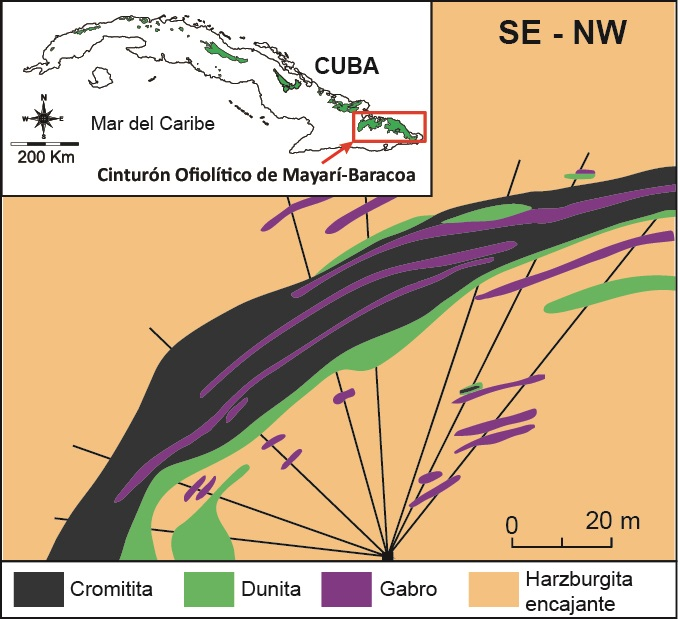
\includegraphics[width=7cm]{Figura1.jpg}}
	\end{figure}
	
	\begin{multicols}{2}
		\section{Resultados}
		Estudios de microscopía óptica y electrónica y microRaman, han permitido identificar diferentes fases en las cromititas: lamelas orientadas de clinopiroxeno (\ref{Fig2}a) y rutilo en la cromita, granos de moissanita en cromita y en la matriz alterada (\ref{Fig2}b), fracturas secundarias selladas con inclusiones de carbono amorfo, serpentina poligonal, lizardita, magnetita, CH\textsubscript{4}, corindón, carbonatos y cuarzo, y granos de Cu nativo y aleación de Fe-Mn en concentrados minerales. 
		También se han encontrado fases similares en cristales de olivino de diques de gabro y dunitas asociadas. En el olivino destacan las inclusiones de magnetita, serpentina y CH\textsubscript{4} (\ref{Fig3}); si bien, también se han encontrado inclusiones aciculares de ilmenita y espinela cromífera (Apéndice \ref{Tabla1}).
	\end{multicols}
	
	\begin{figure}[h]
		\centering
		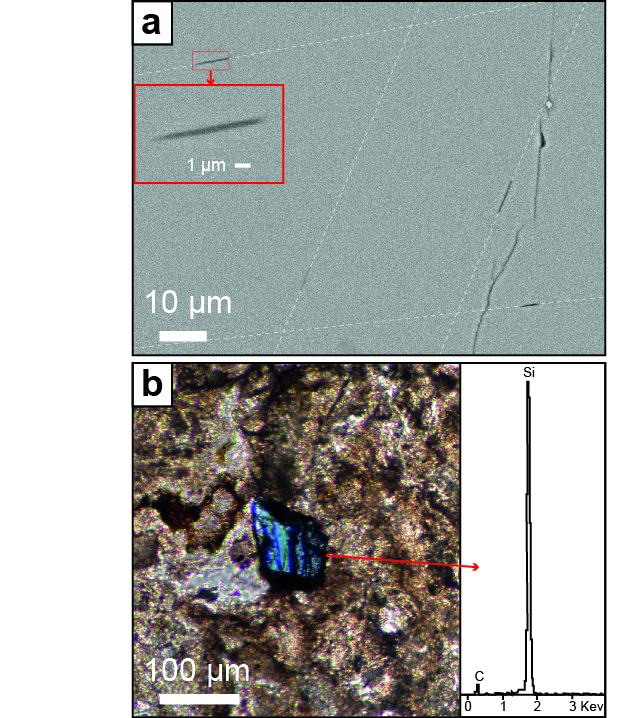
\includegraphics[width=100mm]{Figura2.jpg}
		\caption{\sl a) Lamelas orientadas de clinopiroxeno en cromita (SEM-BSE); b) Grano de moissanita encajado en la matriz alterada de la cromitita (microscopio óptico) y espectro EDS del grano.}
		\label{Fig2}
	\end{figure}
	\begin{figure}[h]
		\centering
		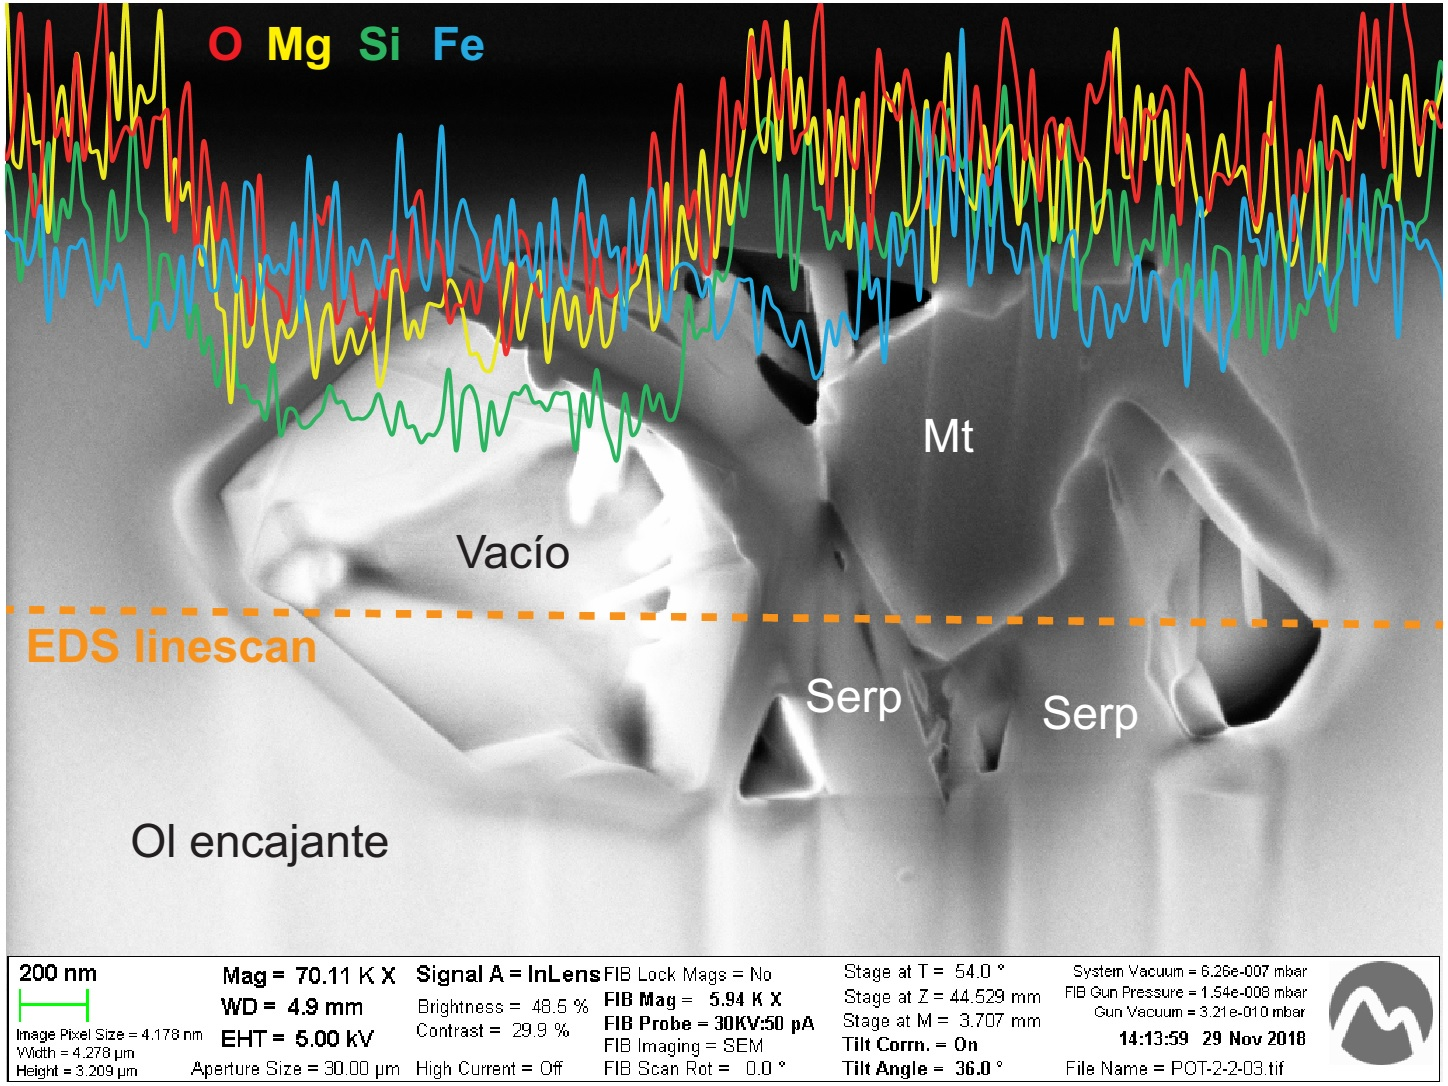
\includegraphics[width=90mm]{Figura3.jpg}
		\caption{\sl Imagen de FIB-SEM de una inclusión con magnetita y serpentina en olivino. Los perfiles indican la abundancia de los elementos en la línea de análisis (EDS linescan)}
		\label{Fig3}
	\end{figure}
		
	\begin{multicols}{2}	
		\section{Discusión y \\conclusiones}
		En la zona estudiada hay evidencias de relación genética entre los diques de gabro no metamorfizados y los cuerpos de cromitita serpentinizados. Esta relación geológica y petrogenética descarta un origen de (ultra)alta presión para los minerales descritos anteriormente. Contrariamente, las lamelas de exsolución (clinopiroxeno y rutilo) se habrían formado durante el enfriamiento de la cromita en el manto. Las fases super-reducidas (p. ej. moissanita, carbono amorfo, Cu nativo y aleación de Fe-Mn) se formaron en microambientes super-reducidos durante la serpentinización en condiciones de baja presión y baja temperatura. Estas condiciones super-reducidas se relacionan con los fluidos C-H-O involucrados en los primeros estadios de la serpentinización de las peridotitas en ambientes submarinos \cite{Golubkova}. En las reacciones de hidratación, el componente H\textsubscript{2}O del fluido se consume para formar fases hidratadas (serpentina), de modo que los fluidos C-H-O pueden alcanzar saturación en C y precipitar fases de C (p. ej. moissanita, carbono amorfo y grafito). El proceso se resume con la siguiente formula:
		\ce{(Fe,Mg)_2SiO_4 + n*H_2O + CO_2 -> Mg_3Si_2O_5(OH)_4 + Fe_3O_4 + CH_4} \cite{Golubkova}.
		\\Estos procesos de serpentinización quedan registrados en las inclusiones de serpentina–magnetita–CH\textsubscript{4} que se encuentran en los olivinos de los gabros. Finalmente, las fases de corteza continental (p. ej. corindón?, cuarzo, circón) podrían representar xenocristales introducidos en el manto por subducción y emplazados en la corteza mediante plumas frías.
\end{multicols}
		
	\bibliography{references}
	\bibliographystyle{apalike}
	 \\
	\begin{appendices}
		\begin{large}
			\bf Apéndice
		\end{large}\\
			\begin{table}[h]
				\caption{Número de inclusiones estudiadas en cada muestra.}
			\begin{tabular}{|c|c|}
				\hline \bf Muestra & \bf Inclusiones estudiadas \\
				\hline
				POT-2(II) & \rm \em 28 \\
				\hline
				L-6-2 & \rm \em 21 \\
				\hline
				86-2-4 & \rm \em 12 \\
				\hline			
				72-2-3 & \rm \em 15 \\
				\hline
			\end{tabular}
				\label{Tabla1}
			\end{table}		
	\end{appendices}
\end{document}